\section{Application structure}
\label{sec:applicationstructure}

%% Graphic of the request cycle to the build pipeline and back
\begin{figure} % h-ere, t-op, b-ottom, p-age
    \centering
    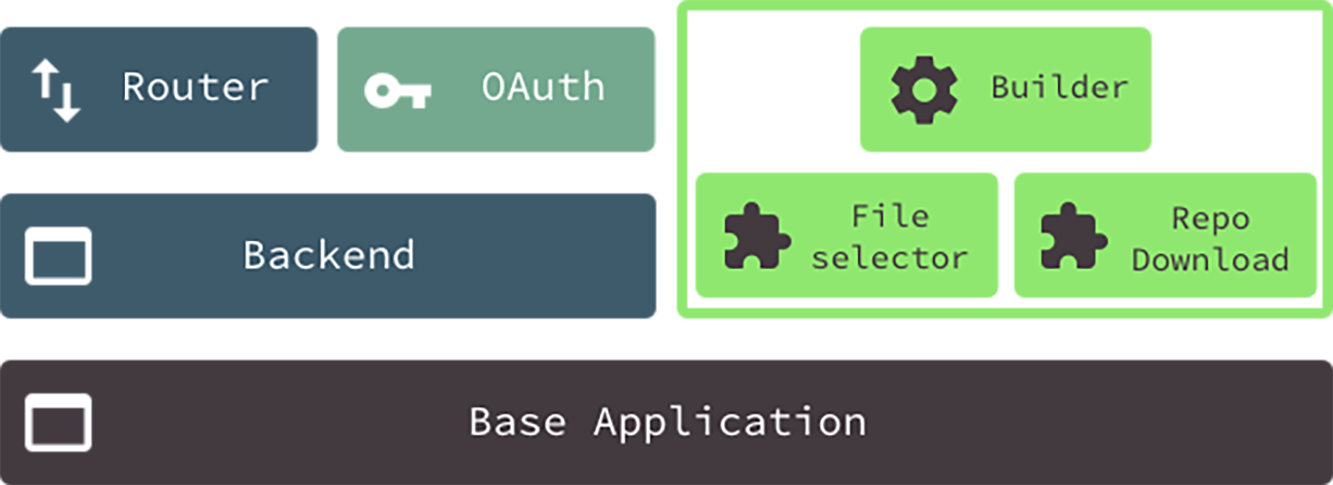
\includegraphics[width=0.9\textwidth]{application_structure.png}
    \caption{A graphic showing the base structure of the implemented application. The \emph{base application} layer serves as foundation, containing necessary libraries for implementing the \emph{HTTP} specifications. The \emph{routing} and \emph{OAuth} layer are responsible for authenticated requests to the endpoints, while the \emph{builder package} is designed as a partly autonomous, loosely coupled rendering service.}
    \label{fig:application_structure}
\end{figure}
%

A basic approach of the project structure may be seen in Fig. \ref{fig:application_structure}. Although this might look still very abstract, the core packages are already clearly visible, while neither the access to the GitHub API, nor the access to the MongoDB is yet visualized.
The graphic can be interpreted as follows:

\begin{itemize}
  \item \emph{Base Application} -- The base structure, consisting of a Node.js environment, together with necessary supporting packages, such as a MongoDB driver and a GitHub API implementation.
  \item \emph{Backend} -- The Express.js ecosystem, responsible for controlling the HTTP subset.
  \item \emph{Router} -- The Express.js router instance, providing all the necessary endpoints for accessing the application's functions.
  \item \emph{OAuth} -- The authentication framework, as theoretically explained in Sec. \ref{sec:foundation-express-oauth}.
  \item \emph{Builder} -- The main build pipeline package consisting of many small plugins for asynchronous handling the process from parsing the configuration to actually building the website.
\end{itemize}

\subsection{Basic setup}
The base application layer is more or less a Node.js stack, covering necessary support features, like reading environment variables or creating various instances of needed modules for the main application flow. It also cares for connecting the service to a MongoDB database, as well as providing a connection framework to the GitHub API.

Furthermore, it holds different database models for user registration, OAuth tokens and build logs. These models are necessary for maintaining a consistent structure on the database collections, thus avoiding custom value checks after fetching entries. Using \emph{Mongoose}\footnote{\url{http://mongoosejs.com} -- Mongoose, ``elegant mongodb object modeling for node.js''}, additional features like manipulation functions and automatic population may be used without depending on other toolsets. One example would be the automatic hashing and comparison of passwords, which is enabled using \emph{pre} hooks on schemas at a certain event (e.g. ``save'')\footnote{\url{http://mongoosejs.com/docs/api.html\#schema_Schema-pre} -- ``Pre'' hook documentation for MongooseJS.}.

\subsubsection{Express.js}
On top of the base application layer, an Express.js setup works as a REST API service. It is configured as first instance in the application's main entry point and is bootstrapped right after the launch of the project. Extending the core module of Express is easy due to the built-in middleware pluggability. A middleware function may get added to the application by binding it to an instance of the app object using an \texttt{app.use()} call \cite{ExpressMiddleware}.

One of the additional middlewares used to extend the app instance is a logging mechanism called ``morgan''\footnote{\url{https://github.com/expressjs/morgan} -- Morgan repository on GitHub.}, which allows a fully customizeable output format for logging HTTP requests and the duration until a response was sent. Another important extension is ``method-override''\footnote{\url{https://github.com/expressjs/method-override} -- Method-override repository on GitHub.}. This module allows the consideration of a \emph{X-HTTP-Method-Override} field in the request header, sent by clients, which are not supporting request types like PUT or DELETE.

\subsubsection{Router}
The middleware concept is designed as a sequential flow of callback functions. Once a request is coming in, the instance is forwarding the data from middleware to middleware until either a response is returned and the middleware chain gets interrupted, or no additional function is left and the instance throws an error.

Thus, the routing mechanism is nothing more than a built-in middleware of Express. It allows for dividing incoming requests based on their URL structure and subsequently assigning them to their respective predefined tasks. These functions again may behave like middleware functions (e.g. for checking authorization, including abstracted functions, imposing pre-conditions, etc\ldots) and therefore expand the callback cycle by additional functionality \cite{ExpressRouter}. A sample implementation of routing middleware may be seen in Listing \ref{list:express-middleware} on p. \pageref{list:express-middleware}.

\subsubsection{Authentication}
Several routes require authentication before being able to access, as a consequence, an automated mechanism handling all necessary steps for securely exchanging user details is inserted in front of the respective routes. Before doing so, the OAuth stack has been implemented -- the \emph{OAuth2orize} package provides an authorization server toolkit for setting up a service implementing the OAuth 2.0 protocol.

The skeleton coming with the package needs to be configured based on the current project's setup, then the instance exposes a middleware, which may be mounted in certain routes \cite{OAuth2orizeGitHub}. After this has happened, the use of the framework may divide the routing configuration into fully accessible routes on the one hand and routes with limited access on the other hand:

\lstinputlisting[caption={A basic router configuration showing the use of an authorization service as a middleware, thus dividing the routes into fully accessible ones (\emph{/all}) and ones with limited access (\emph{/limited} and \emph{/secret}).}, language=JavaScript, label={list:oauth-routes}]{chapters/05-implementation/_support/oauth.js}

From this point on, the client has to provide an access token in the \emph{Authorization} HTTP header using the ``Bearer'' authentication scheme for gaining access \cite[5]{RFC6750}. The service will deny further processing if either an inexisting or already expired access token was provided. In this case, the client has to exchange his/her correct client credentials for a new access token on the authorization endpoint prior accessing the desired endpoint again \cite[41]{hardt2012oauth}.

\subsection{Build pipeline}
\label{sec:structure-buildpipeline}
After the HTTP- and authentication service was built as a user interaction possibility for the upcoming build pipeline realization, the full extent of the necessary API endpoints needed to be defined. Since the OAuth 2.0 framework was already implemented and the access to the GitHub API was prepared as includeable module, only the endpoints responsible for managing and triggering builds, needed to be reserved for the final build service development.

\subsubsection{API integration}

%% Graphic of the first draft of the API
\begin{figure} % h-ere, t-op, b-ottom, p-age
    \centering
    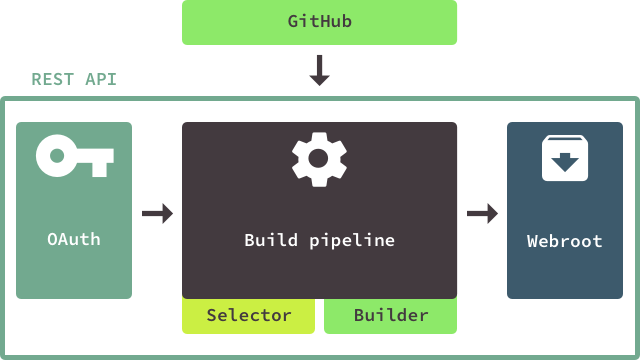
\includegraphics[width=0.9\textwidth]{buildpipeline-api.png}
    \caption{A graphic showing the first draft of the then proposed API cycle. At first the OAuth step should care for authentication, then the build pipeline should be initiated and orchestrate its services to interact with the GitHub API, select files to build and run the build task before saving a rendered version of the webroot, ready for deployment.}
    \label{fig:buildpipeline-api}
\end{figure}
%

From the first draft of an API cycle (as seen in fig. \ref{fig:buildpipeline-api}) to the final structure, a lot of details needed to be tidied up. This was mainly due to the complexity of the build pipeline itself, since one of the biggest challenges were to provide a real non-blocking event loop. By realizing such a non-blocking loop, the client receives an instant, intermediate response, instead of having to queue beforehand, and/or wait until the whole operation finishes. Furthermore, a recurring request for obtaining the build status was enabled using an own endpoint returning informations from the database entry.

The endpoints, which were implemented in favor of user projects, were the following:

\begin{itemize}
  \item \texttt{POST /api/project} -- Creates a project in the database, together with reference to its GitHub data.
  \item \texttt{POST /api/project/:owner/:repo/delete} -- Deletes all references to the project from the database.
  \item \texttt{POST /api/project/:owner/:repo/build} -- Trigger a new build cycle. Returns the reference to the database entry of its build log.
  \item \texttt{GET /api/project/:owner/:repo/status} -- Get the status of the latest build (pending, failed, success).
  \item \texttt{GET /api/project/:owner/:repo/download} -- Download the latest successful build as tar.gz-archive. (e.g. for automated deployments)
\end{itemize}

\subsubsection{Tasks}
As already explained, the build pipeline is realized as a modular concept, consisting of different sub-tasks, bound together in a network of various dependencies to and from each other. Most of these modules are dynamically interlinked with API calls to GitHub, but also with partially strong data modifications of the respective responses.

One after the other, all necessary modules are loaded on request -- to not confuse them by their actual functions, they are divided into three action levels: \emph{engine}, \emph{module} and \emph{support}.

\begin{itemize}
  \item Engine-specific tasks are immediately working for and on the compile actions (e.g. setting up the build pipeline, loading necessary modules, etc\ldots),
  \item Module-specific tasks care for external assistance (e.g. installing modules, compressing rendered output, etc\ldots) and
  \item Support-specific tasks care for engine-specific assistance (e.g. parsing configurations, creating new database entries, etc\ldots).
\end{itemize}

